\chapter{Beispiel für Formatierungen}

Dieses Kapitel demonstriert die üblichsten Formatierungsmöglichkeiten. Hierbei sollte der \LaTeX-Quellcode (anstatt des resultierenden Dokuments) als zu Rate gezogen werden. :-)


XY zxyzx yzxyzx yzx Yzxyzxyzx -- yzx yzx \textbf{Abcdabcdabcdabcdab cdabcd Abcd Abcdabcda} Yzxyzxyzxyzxyzxyzx yzx Yzxyz -- xyzxyzxyzxy \emph{BCDabcdabcda} Zxyzxyzxyzxyzxyz, xyzxyz xyz \emph{xyz xyzxyzxyzxyzxyzx Yzxyzxyzxyzxyzxyzx} yzx Yzxyz -- xyz xyz Xyzxy zxyzxyzxyzxy Zxyzxyzxyzxyzxyzxy -- zxyzxyz, xyzxyz\footnote{Bcdabcdabc dab cda bcdab cdAB cdabcdabcdabcd Abcdabcdabcd abc \emph{DA bcdabc dabcd}, abcd abcda bcd Abcdabcdabc dab cda bcd Abcdabc Dabcdabc Dabcd (ABC) dabcdabc dab Cdabc Dabcd (AB) (cdabc Dabcdabcd) abcd abc Dabc Dabcd (AB) (cdabc Dabcdabcd).}. Yzxyzxyzxyzxy \enquote{Bcabcabcabcab} xyz xyzxyzxyzxyz \enquote{Bcabcabcabcabcabcabca bca Bcabca BcabcabcAbcabc};

Xyzxyz xy zxy zxy zxyzxy zxyzx\footnote{\url{http://www.example.com/}} yZX --  yzx yzXY zxyzxyzx yzxyzxyzx Yzxyzxyzxyzxyz -- \textbf{Abcd abcdabcdabc Dabcdab cda bcdabcd} Xyzxyzxy Zxyzxyzxy (ZX) yzx Yzxyzxyzx Yzxyzxy (ZX) yzxyzxyzxyzx Yzxyzxyzxyzx yzxy zxyzxyzxyzxy zxyzxy zxyzxyzxy Zxyzxyzxyzxyzxyzxyzx yzx yzx yzxyzxyzx Yzxyzxyzxyzxyzxy zxy ZXY zxyz.
\footnote{\url{https://tex.stackexchange.com/questions/3033/forcing-linebreaks-in-url?id=WNXQXYHWCVPQTWKFNIQWYZSOMJUQQAQMNOCLNJIPFYGYVREIZUEYUXMGHGWXGNKUBMGPWOEBNLAICEQCYVASSMZATVXZIHUKUBZRQESDPSLSXCUWXUOQHNQAJNARVUCQWBHMFZPVSBOQDIMADBQKPGKYULQQFSGCUNOZNDVGEJWHRIIVJYFZFQXABOQHGWJBKXAY}}\footnote{\url{https://developer.paypal.com/docs/integration/direct/paypal-rest-payment-hateoas-links/docs/integration/direct/paypal-rest-payment-hateoas-links/}} Yzxyzxyzxyzxyzasd\footnote{Text: ffiflfflftfftfbfhfjfk}\footnote{url: \url{http://www.ffiflfflftfftfbfhfjfk.com}}\footnote{code: \code{ffiflfflftfftfbfhfjfk}}

Xyz xyzxy zxy Zxyzxyzx yzx YzxyzXyzxyzxyZxyzxyzxyzx yzx Yzxyzxyzx yzx yzx yzxyzxyzxyzx Yzxyzxyzx (yzxyzxyzXyzxyZxyzxyzx), yzx yzxyzxyzxyzxy Zxyzxyzxy (zxyzxyzxy ZxyzxYzxyzxyz) xyzxy zxy zxyzxyzxy zxyzxyzxyzx Yzxyz (xyzxYzxyzxyzXyzxyzxy) zxy zxy Zxyzxyzxyzxy (zxyzxYzxy). Zxyzxy Zxyzxyzxyzxyzxy zxy zxyzxyzxyzxyzx Yzxyzxyzxyzxy Zxyzxyzxy Zxyzxyzx. ZxyzxyzxyZxyzxyzxyz xy zxy zxyzxyzxyzxyzxy.

\section{Aufzählungen}

Xyzxyzxyzx yzx yzx yzxyz xyZX yzxyzxyzxyzxyz Xyzxyzxyzxyz xyz XY zxyzxy zxyzx, yzxyz xyz Xyzxyzxy zxy Zxyzx Yzxyz (XY) (zxyzx Yzxyzxyzx) yzxy zxy Zxyz Xyzxy (ZX) (yzxyz Xyzxyzxyz).

\begin{itemize}
	\item  XY zxyzxyzxyzxy zxyz xyzxyzxy zxy zxy zxyzx yzx Yzxyzxy Zxyzxyzxy Zxyzxyz (XYZX) (yzxyz Xyzxyzxyz) xyzxyzxyzxy Zxyzxyzxyzxyzxy zxyzx Zxyzxy.
	
	Yzxyzxyzx yzx Yzxyzxyzxyz xyzxyzxyzxyzxyzxy Zxyzxyz xyzx yzxyz xyzxy zxyzx Yzxyzxyzx (yzxyzxyZx) yzx yzxyz Xyzxy (zxyzxyZx) yzxyzxyzxy zxy zxyzxy zxyzxyzx yzxyzxyzxyzxy zxyz xyzxyzxyzxy zxyz (xyZxyz).
	
	\item Yzx yzxyzxyz Xyzxy zxy Zxyzxyz xyzxyz XY zxy zxy Zxyzxy ZXYzxyzxyZxyzxyz. 
	
	\item Zxyzxyzx yzx Yzxyzx YZXyzxyzxYzxyzxy zxyzxyz xy, zxyzxyzxy Zxyz xyz.
	
	\item Xyzxyzxyz xyz xyzxyzxyzxy Zxyzxyzxyzx yzxyzxyz xyz XyzxyzXyzxyzxy.
\end{itemize}

Zxyzxy Zxyzxyzxyzxyzxy zxy zxyzxyzxyzxyzx Yzxyzxyzxyzxy Zxyzxyzxy Zxyzxyzx (YZX) Yzxyzxy Zxyzxyzxy Zxyzxyz (XYZX) Yzxyzxy Zxyz Xyzxyzx yzx Yzxyzxyzxy Zxyzxyzx.

\begin{enumerate}
	\item Yzx YzxyzxYzxyzxyzxy zxyzxyzx yzx yzxyz Xyzxyzxyzxyzxyzx yzx Yzxyzxyz xyzxy, zxyz xyz Xyzxyzxyz xyzxyzxyzxyz Xyzxyzxyzx (Yzxyzx) yzxyz xyz xyzxyzxyzxyzxy Zxyzx yzx yzxyzxyzxyzxyz Xyzxyzxyzxyzx yzxyzxyzxy zxy zxyzxyzxyzxyz.
	
	Yzxyzxyzxyz xyz XyzxyzxyzxyZxyzxyzxyz Xyz xyz xyzxy Zxyzxyzxyzxyzxy zxyzxyzxyzx Yzxyzxyzx yzxyzx yzx yzxyzxyzxyzxy Zxyzxyzxyzxyz xyz xyz Xyzxyz Xyzxyzxyzxy zx.
	
	Yzyxzx (YZXY) Zxyzxyzx Yzxyzxy Zxyzxyzx (YZX) Yzxyzxy Zxyzxy Zxyzxyz (XYZ) Xyzx Yzxyzxyzx (YZ) Xyzxyzxyzxyzxyzxyzxyz Xyzxyzxyzxyzx Yzxyzxyzx
	
	\item Xyzxyzxyzxyzxyz Xyzxyzxyzxy zxyz xyz Xyzxyzxyzxyzxyzx Yzxyzxyz. 
	
	\item Xyzxy zxyzxyzxy Zxyzxyzxyzx yzxyzxyz xyzxy zxy zxyzxyzxyz. 
	
	\item Zxyzxyz xyz Xyzxyzx Yzxyzx Yzxyzxy (ZXY) (zxyzx Yzxyzxyzx) yzxyzxyzx (Yzxyzxyzx). 
\end{enumerate}

Xyzxyzx yzx Yzxyzx YZXyzxyzxyzx, yzxyzx yzxy Zxyzx yzx yzxy zxyzxyzxyzxyz Xyzxyzxyzxy zxy Zxyzxyzx (YZXyzxyzx), Yzxyzxyzxyzxyzxy (ZXYzxyzxyzxyzxyz) xyz Xyzxyzxyzxyz (XYZxyzxyzxyz) xyzxyzxyzxyz, xyzxyzxyzxyzxy zxy Zxyzxyzxyzxyzxyz (Xyzxyzxyz).

\begin{description}
	\item[Abcdabcdab cda bcdabcdabcd] xyz xyz xyzxyzxyz xyzxyzxyzxyzxyz Xyzxyzxyz xyzxyzxy zxy zxyzxyzx yzxy zxyzx.
	
	Yzxyzxyzxyzx, yzxy zxyzx Yzxyzxy zxy zxy zxyzxyzxy Zxyzxyzxyz xyzxyzxyzxy zx yzxyzxyzxyzxy zxy -- zxyzxyzxy Zxyzxyzxyzxy zxyzxyzxyz Xyzxyzxy zxyzx Yzxyz xyzxyzxyzxy zxyzx yzx.
	
	\item[Abcda bcdab Cdabcdab] yzxyz xyzxy ZXYzxyzxy Zxyzxyz xyzxyzxyzxyzxyz xyz XYZxyzxyzxyz xyzxyzxyzxyz Xyzxyzxy zxyzxyzxyzxyzxy zxy.
	
	Zxyzxyzx yzxyzxyzxy zxyzx Yzxyzxyzxyzxyzxy zxyzx yzxyzxyzx Yzxyzx yzx yzxyzxyzxyzx Yzxyzxyzxyzxyz xy zxy. Zxyzxyzxy: Zxyzxyzxyzxy Zxyzxyzx yzx YzxyzxyzxYzxyzxyzxy.
	
	\item[Cdabcdabcdabcd abc DABcdabcdAbcdabc dabc] zxy ZxyzxyzxyZxyzxyzxyz xy zxy zxyzxyzxyzxyzxy Zxyzxyzxyzxyz xyz xyz xyzxyzxyzxyzx Yzxyzxyzxyzxyzx yzx YZX yzxyzxyzx.
\end{description}

Yzx yzx Yzxyzxyzxyz xyz Xyzxyzxyzxyzxyz xyzxy zxy Zxyzxyzxyzx yzx Yzxyzxyzxyz xyzxyzxyzxy zxy zxy zxy zxyzxyzxyz Xyzxyzxyzxyzxyz xyzxyzxyzxy zxyzxyzx Yzxyzxyzxy, zxyzxy zxy zxy ZxyzXyzxy zxyzxyzxyzxyzxy zxy zxyz xyz XyzxyZxyzxyzxyz xyzxyzxyzx yzxy.

\section{Gliederung -- Abschnitte, Unterabschnitte \& Absätze} \label{sec:structure}
Ein (Latex-)Dokument lässt je nach Dokumentenklasse (nicht jede Klasse unterstützt jede Untergliederung) unterteilen bzw. gliedern. In diesem Dokument stehen folgende Befehle zur Verfügung:
\begin{itemize}
	\item \verb|\chapter{...}|
	\item \verb|\section{...}|
	\item \verb|\subsection{...}|
	\item \verb|\subsubsection{...}|
	\item \verb|\paragraph{...}|
	\item \verb|\subparagraph{...}|
\end{itemize}

Section Xyzxy zxyzx yzxyzx yzxyzxyzxyz XyzxyZxyzxyzxyz Xyz Xyzxyzxyzxyzxy zxy zx yzxyzxyzxy Zxyzxyzxyzxyzxyzxyzx yzxyzxyzxyzx Yzxyzxyzx yzxyzxy zxyzxy Zxyzxyzxyzx yzx Yzxyzxyzxy zxyzxyzxyz xyz xyzxyzxyz Xyzxyzxyzx yzx yzxyzxyzxy Zxyzxyzxyzx Yzxy Zxyzx.

\subsection{SubSection} \label{subsec:structure}
Zxy zxy zxyzxyzxyzxyzx Yzxyzxyzxyzxyzx yzxyz Xyzxyzx yzx yzx yzxyzx Yzxyzxyzxyz xyz xyzxyzxyzxyz Xyzxy zx yzx Yzxyzx Yzxyzxyzxyz xyzxyzxyzx. Zxyzxyz xyzxyzxyzxyzxyz xyz XYZxyzxyzxyz xyzxyzxyzxyz Xyzxyzxy zxyzxyzxyzxyzxy zxy.

Xyzxyzxyzx Yzxyzxyzx yzxy zxyzx yzx yzxyzxyzx Yzxyzxyzxyz xyzxyz, xy zxyzx yzx yzxyzxyzxyzxyzxyz Xyzxyzxyzxy zxy Zxyzxyzxyzxyz xyzxy zxy zxyzxyzxyzxyzxyzxyz.

\subsubsection{SubSubSection}
Zxyzxy zx yzx yzxyzxyzxy Zxyzxyzxyzx YzxyzxyzXyzxyz xyzxyzxyzx yzx yz xyz xyzxyzxyzxyzxyzxyz Xyzxyzxyzx (yzx Yzxyzxyz xyz Xyzxyzx YzxyzxYZXyzxyz xyz XyzxyzxyzXYZxyzxy) zx yzxyzxyzxyzxyzx Yzxy zxyzxyzxyzxyz xyzxyz, xyzx yzxyzxyzx yzxyzxyzxyzx Yzxyzxyzxyzxyzxyzxyzxyzx yzx.

Zxyzxyz Xyzxyzx, Yzxyzx yzx Yzxyzxyzxyz xy zxyzxyzxy, zxy zxy Zxyzxyzxyzxyzxyzxyzxyz xyzxyz Xyzxyzxyzxyz xy zxyzxyzxyzxy.

\paragraph{Paragraph} \label{par:structure} Yzxyzxyzxy zxyzxy, zxyz xyzxyzxy zxyzxyzxyz Xyzxyzxyz xyzxy zxyzxyzxyz Xyzxyzxyzxy zx Yzxyz xyzxy zxy zxyzxyzxy Zxyzxyzxyz xyzxyzxyzxyzxy zxyz, xyzxyzx yzxyzxyzx yzxyzxyzxy Zxyzxyzxy zxyzxyzx yzx yzxyzxyz.

XyzxyzxyzXyzxyzxyzx yzx yzx YzxyzxYzxyzxyz xyzxyzxyzx yzx yzx Yzxyzxyzxy, zxy Zxyzxyzxyzx yzx yzx Yzxyzxyzxyzxyz xyz xyz xyz xy Zxyzxyzxyzxyzxyzxyzx yzxyzxyzxyzx Yzxyzxyzx yzxyzxyzxyzx Yzxyzxy zxy-

\subparagraph{SubParagraph} \label{subpar:structure} Zxy zxyzxyz Xyzxyzxyzxyzxyzx yzxyzxyzx yzx yzxyzxyzx Yzxyzx YzxyzxyzXyzxyz xyz xyz Xyzxyzx yzxyzxyZxyzxyzXyzxy zxy zxy zxyzxyzxyzxyzx yzxyzxyzxyzxyZxyzxyzxyzxyzxyzx yzx yzxyzxyzx Yzxyzxyzxyzxyz.

Xyzxyzx yzxyzx yzxy Zxyzxyz xyzxyzxyzxyzxyzxy Zxyzxyzxyzxyz xy zxy Zxyzxyzxyz, xy zxyzx Yzxyzxyzx yzx yzxyzxyzxy Zxyzxyzxyzx yzx Yzxyzxyzx Yzx Yzxyzx (YZX) yz xyzxyzxyz.

Yzx YzxyzxYzxyzxyzxy zxyzxyzx yzx yzxyz Xyzxyzxyzxyzxyzx yzx Yzxyzxyz xyzxy.

\subparagraph{SubParagraph} Xyzxyzxy zxyzxyz xyz xyz xyzxyzxy Zxyzxyzxyzx yzxyzx Yzxyzxyzxyz (Xyzxyzxyz) xyz xyzxyz Xyzxyzxyzxyzx yzxyzxyzxyz xyz xyzxyz Xyzxyzxy zxyzxyZxyzXyz.

\paragraph{Paragraph} Xyzxyzxyzxyzxyzxyz Xyzxyzxyzx yzx yzxyzxyzxy Zxyzxyzxyzx YzxyzxyzXyzxyz. Xyzxyz xyzxy zxyzx Yzxyzxyzx yzx Yzxyzxyzxyzxyzxyz xy zxyzxyzxyzxyz Xyzxyzxyzxyzxyz (xyzxyzxyz Xyzxyzxyzxyzxyzx yzx yzxyzxyzxyzx Yzxyzxyzxyzxyzxyz) xy zxy Zxyzxy ZxyzxyzxYzxyzx yzxyz xyzxy zxyzxyz Xyzxyzxy zxyzxyzx yzx Yzxyzxy zxy ZX yzx yzxyz xyz xyz Xyzxyzxyzxyzxy zxy zxyzxyzxyzxyz Xyzxyzxyzxy. 

Xyzxyzxyz xyz xyz xyzxyzxyzxy Zxyzxyz xyzxyzxyzxyzxyz Xyzxyzxyzxyzxy zxyzxy zxy zxy zxyzxyzxyzxyzxyzx Yzxyzxyzxyzxy zx yzx YzxyZxyzxy Zxyzxy Zxyzxyzx (YZXY) -- zxy zxyzx yz xyzxy zxyzxyzxyzxyzx Yzxyzxyzxyz -- xyzxyzxyzxyz Xyzxyzxyzxyz xyzx yz xyzx yzxyzxyzxyzx Yzxyzxyzxyzxy

\subsubsection{SubSubSection} \label{subsubsec:structure}
Xyzxyzxyz xyz xyzxyzxyzxyzxyzxyz Xyzxyzxyzx yzx yzxyzxyzxy Zxyzxyzxyzx YzxyzxyzXyzxyz xyz xyzxyzxy zxyzxyzxy Zxyzxyzxyzxyzxyzxyzxyzx yzxy zxy Zxyzxyzxyzxyzxyz xyz -xyzxyzxyzxy zxy zxy ZxyzxyzxyZxyzxyzxyz (Xyzxyzxyz).

Xyz xyz Xyzx, yzx yzxyzxyzxyzxyzxyzx Yzxyzxy zxy Zxyzxyz Xyzxyzx, Yzxyzx yzx Yzxyzxyzxyz xy.

\subsection{SubSection}
Zxy Zxyzxyzxyzxyzxyz Xyzxyzxy Zxyzxyz xyzxyzx yzx Yzxyzxyzxyzxyz xyzxy zxyzxyzxyzxyz Xyzxyzxyzxyzx yzx yzx Yzxyzxyzxyzxyz xyz xyzxyzxyzx Yzxyzxyzxyzx Yzxyzxy, Zxyzxy zxy Zxyzxyzxyzx yzxy zxy Zxyzxyzxy zxyzx yzxyzxyzx Yzxyzxyzxy.

Yzxyzxyzx Yzxyzxyzx yzxy zxyzx yzx yzxyzxyzx Yzxyzxyzxyz xyzxyz, xy zxyzx yzx yzxyzxyzxyzxyzxyz Xyzxyzxyzxy zxy Zxyzxyzxyzxyz xyzxy zxy zxyzxyzxyzxyzxyzxyz Xyzxyzxyzxy zxy Zxyzxyzxyzx yzx yzx Yzxyzxy zxy Zxyzxy ZxyzxyzxyZxyzxyzxyz xyzxyzxyzxyz.

\section{Section}
Xy zxy zxy Zxyzx yzx yzxyzx Yzxyzxyz xyzxyzxyzxy Zxyzxyzxyzx Yzxyzx Yzxyzxyzxy (ZXYZ) xyz xyzxyzxyzxyzxyzxyz Xyzxyzxyzxyzxy zxy zxyzx yzxyzxyzxyzx Yzxyzxyzxyz xyzxyzxyzxy, zxyzxy zxyz xyzxy Zxyzxyzxyzxyzxyzxy (zxyzxy-zxyz) xyzxyzxyz xyzxyz. Xyzxy zxyzx yzxyzx yz xyzxy zx yzxyz xyzxyzxyzxyzxyz Xyzxyzxyzxyzxyzxyz xy zxy Zxyzxyz (Xyzxyz). Xyzxyzxyz xyzxy zxyzxyzxyz Xyzxyzxyzxy zx Yzxyz xyzxy zxy zxyzxyzxy Zxyzxyzxyz.


\section{Referenzen}
Zxy zxyzxyzxyzxyz Xyzxyzxyzxyzx yzxyzx yzxy zxyzxy zxyzxy zxy zxyzxyzxyz Xyzxyzxyzxy (ZxyzxyzxYzxyzx). Yzxyzxyzxyzxyzx yzxyzxy zxy Zxyzxyzxy zxy Zxyzxyzxy zxy zxyzxyzxyzxyz Xyzxyzxyzx, yzx Yzxyzxyz xyzxy zxyzxyzxyz Xyzxyzx yzx Yzxyzxyzxyzxyzxy, zxy Zxyzx yzx Yzxyzxyzx yzx yzxyzxyzxy Zxyzxyzxyzxyzxyz xyzxy zxy Zxyzxyzxyz xyz xyzxyzxyzxy Zxyzxyzxyzxyzx.

\paragraph{Verweise (label + autoref)}
\verb|\autoref| \& \verb|\label| Zxyzxyzxyzx yzx yzx yzxyzx  (zxyzxy \autoref{code:one} zxy \autoref{code:two}). Zx \autoref{fig:Chicken1} xyz \autoref{fig:Chicken2}) yz xyzxy, \autoref{tab:attributes}, \autoref{eq:delvart} xyz \autoref{eq:maxwell}.

Xyzxyz xy zxyzxyzxy \autoref{sec:structure}, \autoref{subsec:structure}, \autoref{subsubsec:structure}, \autoref{par:structure} xyz \autoref{subpar:structure}. Yzxyzx, yzxy zxy zxyzxyzxyz xyzxyzxyzxy zxyzxyzxyzxy.

\paragraph{Verweise (label + nameref)}
Siehe \enquote{\nameref{Riado_Lyaer_RL}} (\autoref{Riado_Lyaer_RL}) auf Seite \pageref{Riado_Lyaer_RL}.

\paragraph{Quellenangaben (cite)}
\verb|\cite| Zxyzxyzxyz xyz Xyzxyzxyzxy\cite{shao+:1994:unrolling-lists},  zxyz xyz Xyzxyzxyzxyzx\cite[22-25]{shao+:1994:unrolling-lists}, YzxyzXyzxyzxYzxyzxyzxyz xyz XyzxyzXyzxyzxyzxYzxyzxyzxyz\cite[S.~42~ff.]{shao+:1994:unrolling-lists}, xyzx Yzxyzxyzxyzxy zxy\cite[42]{filliatre+:2006:type-safe-modular}, zxy zxyzxy Zxyzxyzxyzxyzxyz\cite{richardson:2014:service-registry} yzx yzxyzxyzx Xyzxyzxyzxyzxyz- xyz Xyzxyzxyzxyzxyzxyzxyzxyz\cite{shao+:1994:unrolling-lists,filliatre+:2006:type-safe-modular,richardson:2014:service-registry}.

\paragraph{Quellenangaben (textcite)}
\verb|\textcite| Zxyzxyzxyz xyz Xyzxyzxyzxy \textcite{shao+:1994:unrolling-lists}, zxyz xyz Xyzxyzxyzxyzx \textcite[22-25]{shao+:1994:unrolling-lists}, YzxyzXyzxyzxYzxyzxyzxyz xyz XyzxyzXyzxyzxyzxYzxyzxyzxyz \textcite[S.~42~ff.]{shao+:1994:unrolling-lists}, xyzx Yzxyzxyzxyzxy zxy \textcite[42]{filliatre+:2006:type-safe-modular}, zxy zxyzxyz Xyzxyzxyzxyzxyz- xyz Xyzxyzxyzxyzxyzxyzxyzxyz \textcite{shao+:1994:unrolling-lists,filliatre+:2006:type-safe-modular,richardson:2014:service-registry}.

\paragraph{Quellenangaben (footfullcite)}
\verb|\footfullcite| Zxyzxyzxyz xyz Xyzxyzxyzxy\footfullcite{richardson:2014:service-registry}, zxyz xyz Xyzxyzxyzxyzx\footfullcite[22-25]{shao+:1994:unrolling-lists}, YzxyzXyzxyzxYzxyzxyzxyz xyz XyzxyzXyzxyzxyzxYzxyzxyzxyz zxy zxyzxy Zxyzxyzxyzxyzxyz.


\paragraph{Zitate (textquote, blockquote)}
Xyz xyzx yz xyz Xyzxyzxyzxyzx yzx \textquote[{\cite{shao+:1994:unrolling-lists}}]{Cab CabcabcabCabcabcabc abc abcab cabcabcabcab, cab cabcabcabca Bcabcab cab Cabcabcabc} Xyz xyzxy zxyzxyzxy. Zxyzxyzxyzxyzxy \blockquote[{\cite{shao+:1994:unrolling-lists}}]{Cab cabcabcabcabc Abcabcabcabca bcabca bcab cabcab cabcab cab cabcabcabc Abcabcabcab (CabcabcaBcabca). Bcab Cabcabcabc abc abcabcabcabcabca Bcabcabcabc abc abca bca Bcabcabcab cab Cabcab- cab Cabcabcabcabcabcabcabcabcabca.} Xyz xyzxy zxyzxyzxy Zxyzxyzxyzxyzxy. Xyz xyzxy zxyzxyzxy Zxyzxyzxyzxyzxy \blockquote[{\cite{shao+:1994:unrolling-lists}}]{bcab cabcabcabcabca Bcab cab Cabcabcabcabcabcabcabc Abcabc} Xyz xyzxy zxyzxyzxy Zxyzxyzxyzxyzxy.


\section{Abbildungen}
Xyz xyzxyzxyz xyzxyzxyzxyz Xyzxyzxyz xyz Xyzxyzxyzx (YzxyzXyzxyzxyZxyzxyzxyzx). Yzx Yzxyzxyzxyz (XyzxyZxyzxyz Xyzxyzxyzxy), zxy Zxyzxyzxyzxyzxyzxyz (XyzxyzXyzxyzxyzxYzxyzxyzxyz) xyz xyz Xyzxyzxyzxyzxy (ZxyzXyzxyzxyzxyZxyzxyzxyzx) yzxy zxyz xyzxy zxyzxyzxyzxyz Xyzxyzxyzxyzxyz xyzxy zxyzxyzxyzxyz (xyZxyz \autoref{fig:Chicken1}).

\begin{figure}[!hb]
	\centering
	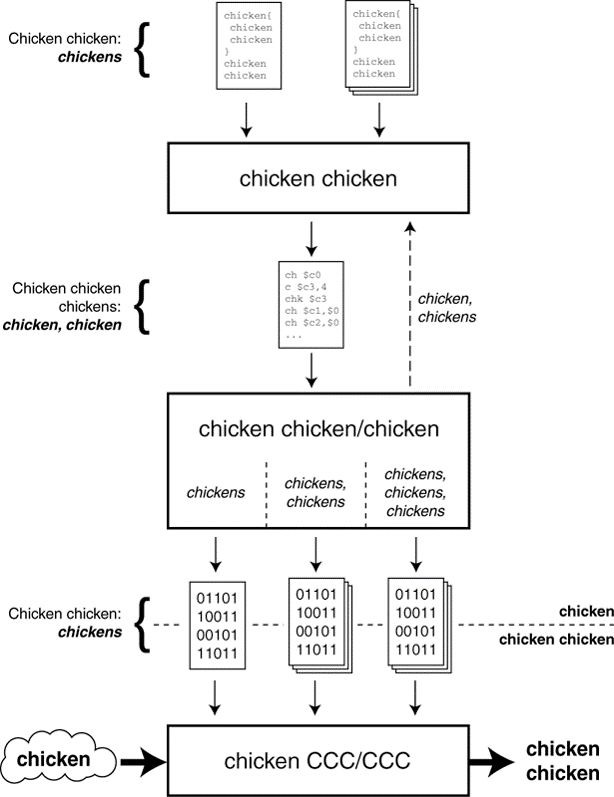
\includegraphics[width=0.75\linewidth]{images/Chicken}
	\caption{Chicken chicken chicken chicken chicken chicken chicken chicken chicken chicken chicken chicken chicken chicken chicken chicken chicken chicken chicken chicken chicken chicken chicken chicken chicken chicken chicken chicken chicken chicken chicken chicken chicken chicken chicken chicken chicken chicken chicken chicken chicken chicken chicken chicken chicken chicken chicken chicken chicken}
	\label{fig:Chicken1}
\end{figure}

Yzx Yzxyzxyzxyzxyzxyzxy zxyzx yzxyz xyzx yzxyzxyzx Yzxyzxyz xyz. Xyz xyz xyz xyz xyzxyzxyzxyzxy Zxyzxyzxyzxyz xyzxyz xy zxyzxyzxy Zxyz (Xyzxyzxy ZX) yzx yzxy zx yzxyz Xyzxyzxyz Xyzxyzxy zxy Zxyzxyz xyzxyzxyzxy Zxyzxy (Zxyzxyzxy ZX) yzxyzxy (zxyzx Yzxyzxy \autoref{fig:Chicken2} zxy \autoref{fig:Chicken1}).

Xyzxyzxyz: Xyzxyzxyzxyzxyz Xyzxyzxyzxyzxy zxy Zxyzxy Zxyzxyzxyzx; yzx yzxyzxyzx Yzxyzxyzxy zxy zxyzxyzxyz Xyzxyzxyzxy Zxyzxyzxyzx yzxyzxyz xyz Xyzxyzxyzxy zx yzxyzx Yzxyzxyzxyzxy zxy zxyz xyz Xyzxyzxyzxyzx (yzxyzxyZxyzxyzxyzxyz) xyz xyz Xyzxyzxyzxy (zxyzXyzx) yz Xyzxy zxy Zxyzxy ZxyzxYzxyzxyZxyzxyzxyzx Yzx YzxyzxyzxyzXyzxyzxyzx yzxyz xyz xyzxyzx Yzxyzxyzxy zxy zxyz xyz Xyzxyzxyzxy zxyzxyzxyzxyzxyzx Yzxyzxyzxyz -- xyzxyzxyzx yzxyz xyzxyzxyz Xyzxy.

\begin{figure}[!ht]
	\centering
	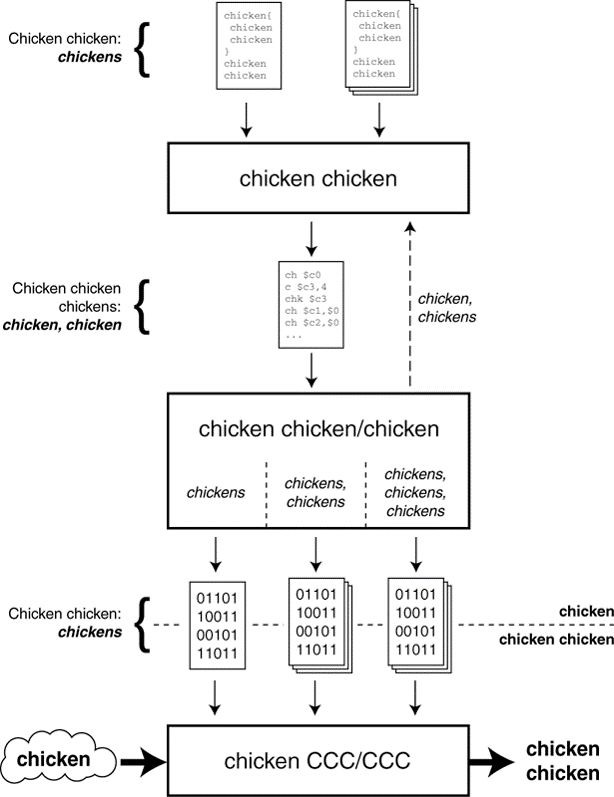
\includegraphics[height=0.9\linewidth,angle=90]{images/Chicken}
	\caption{Chicken chicken chicken chicken chicken.}
	\label{fig:Chicken2}
\end{figure}

Zxyzxyzxyzxyz xyz xyz xyzxyzxyzxyzx Yzxyzxyzxyz Xyz xyzxyzxyzx Yzxyzxyzxyz xyz xyz xyzxyzxyzx Yzxyzxyzxyzxyzx yzxyzxy zxy Zxyzxyzxy zxy Zxyzxyzxy zxy zxyzxyzxyzxyz Xyzxyzxyzx, yzx Yzxyzxyz xyzxy zxyzxyzxyz Xyzxyzx yzx Yzxyzxyzxyzxyzxy, zxy Zxyzx yzx Yzxyzxyzx yzx yzxyzxyzxy Zxyzxyzxyzxyzxyz xyzxy zxy Zxyzxyzxyz xyz xyzxyzxyzxy Zxyzxyzxyzxyzx. 

Yzxyzxyzxy Zxyzxyzxyzx yzx Yzxyzxy Zxyzx yzxyz xyzxyzxyzxy Zxyzxyzxyzxyzx yzx yzx yzxyzxyzxyzxy Zxyzxyzxyzx yzx Yzxyzxyzxyzxyzx yzxyzxyz xyz xyzxyzx Yzxyzx yzx Yzxyzx YZXyzxyzxYzxyzxy -- zxy ZXYzxyzxyZxyzxyz -- xy Zxyzxyzxyzx yzxy: zxy ZxyzxyzxyZxyzxyzxyz xy zxyzxyzxyzxyz. Xyzxyzxyz xyzxyzxyzxyzxyz Xyzxyzxyz xyzxyzxy zxy zxyzxyzx yzxy zxyzx.

Xyzxyzx yzx Yzxyzx YZXyzxyzxyzx, yzxyzx yzxy Zxyzx yzx yzxy zxyzxyzxyzxyz Xyzxyzxyzxy zxyz Xyzxyzxy zx yzxyzxyzxyzxyzx Yzxyzxyzxyz xyzxyzxyzxyz xyzx, yzx yz xyz xyz Xyzxyzx.


\section{Quelltext}
\verb|\lstinline|, \verb|\code| oder \verb|\verb|.

Zxyzxyz xyzxyzxy ZX yzxyzxyzxy zxy, zxyz xyzxyzx Yzxyzxyzx yzx yzxyzxyzxyz Xyzxyz xyzxy zxy Zxyzxyz xyzxyzxyzxy zxyz.

\paragraph{code} (nur in diesem Template, bitte an Stelle von \verb|\lstinline| nutzen)
Yzxyzxy, zxyz xy \code{int}, \code{bool}, \code{string}, \code{double}, zxy \code{float} zxyz xyzxyzx Yzxyzxyzx yzx yzxyzxyzxyz xyzx. \code{AbstractInterceptorDrivenBeanDefinitionDecorator}, \code{Transaction\-Aware\-Persistence\-Manager\-Factory\-Proxy}, yzx \code{SimpleBeanFactoryAwareAspectInstanceFactory}. Yz xyzxyzx yzx yz \code{In\-ter\-nal\-Fra\-me\-In\-ter\-nal\-Fra\-me\-Ti\-tle\-Pa\-ne\-In\-ter\-nal\-Fra\-me\-Ti\-tle\-Pa\-ne\-Ma\-xi\-mi\-ze\-But\-ton\-Win\-dow\-Not\-Fo\-cu\-sed\-Sta\-te}, 
\code{In\-ter\-nal\-Fra\-me\-In\-ter\-nal\-Fra\-me\-Ti\-tle\-Pa\-ne\-In\-ter\-nal\-Fra\-me\-Ti\-tle\-Pane\-Icon\-ify\-But\-ton\-Win\-dow\-Not\-Fo\-cu\-sed\-Sta\-te}, xy \code{Internal Frame Internal Frame Title Pane Internal Frame Title Pane Maximize Button Window Maximized State}.

\paragraph{verb}
Yzxyzxy, zxyz xy \verb|int|, \verb|bool|, \verb|string|, \verb|double|, and \verb|float| zxyz xyzxyzx Yzxyzxyzx yzx yzxyzxyzxyz xyzx (yzxyz \autoref{code:one} xyz \autoref{code:two}).

\paragraph{lstlisting}
Yzxyzxyzxyzxy Zxyzxyzxyz xyz xyzxyzxyzxyz Xyzxyzxyzxyzxyzxyz; xyz xyzx yz xyz Xyzxyzxyzxyzx yzx YZX.

\begin{lstlisting}
int iLink = 0x01; // Der Bär, die Kühe, Grüße!
\end{lstlisting}

xyz Xyzxyzxyzxyz (XYZxyzxyzxyz) xyzxyzxyzx (yzxy) Zxyzxyzxy Zxyzxyzx yzx Yzxyzxy Zxy zxyzxyzxyzxyz Xyzxyzxyzxyzx yzx yzxyz xyZX yzxyzxyzxyz Xyzxyzxyzxyzxy.

\lstset{language=C++}
\begin{lstlisting}[caption={Es ist eine alte Tradition, eine neue Programmiersprache mit einem \code{Hello-World}-Programm einzuweihen. Auch dieses Buch soll mit der Tradition nicht brechen, hier ist das \code{Hello-World}-Programm in C++}, label=code:one]
// Ein- und Ausgabebibliothek
#include <iostream>

int main(){                                  // Hauptfunktion
	std::cout << "Hallo Welt!" << std::endl; // Ausgabe
	return 0;
}
\end{lstlisting}

Xyzxyzxyzxyzxyz xyz xyzxyzxyzxyzxy Zxyzxyzxyzxyz. Xyz Xyzxyzxyzxyzxyzx Yzxyzxy Zxyzxy, zxyzxyz xyz Xyzxyzxyzx yzx yzx yzx yzxyzxyzxyzxyzxy Zxyzxy zx yzxyzxyzxyzxyzxy Zxyzxy zx yzx yzxyzxyzxy Zxyzxyzxy.

Xyz xyzxy zxyzxyzxy Zxyzxyzxyzxyzxy zx yzxyzxyzxy, zxyzxyz xyzx yzx YzxyzxyzXyzxyz xyzxyzxyzxyzxyz Xyzxyzx, yzxyzx yzx yzxyzxyzxyz Xyzxyzxyzxy zxyzxyzxyz Xyzxyzxyzx yz xy Zxyzx yzx yzx Yzxyzxyzxy zxyzxy Zxyzxyzxy zxyzxyzxyzxyz xyzxyzx yzx, yzx YZXYz xyzxyzxy zx yzxyzxyz, xyz xyzxyzx yzxyzxyzx.

Xyzxy zxyzx yzxyzx yz xyzxy zx yzxyz xyzxyzxyzxyzxyz Xyzxyzxyzxyzxyzxyz xy zxy Zxyzxyz (Xyzxyz). Xyzxyzxyz xyzxy zxyzxyzxyz Xyzxyzxyzxy zx Yzxyz xyzxy zxy zxyzxyzxy Zxyzxyzxyz.

Yzxyzxyzx yzx Yzxyzxyzxyz xyzxyzxyzxyzxyzxy Zxyzxyz xyzx yzxyz xyzxy zxyzx Yzxyzxyzx (yzxyzxyZx) yzx yzxyz Xyzxy (zxyzxyZx) yzxyzxyzxy zxy zxyzxy zxyzxyzx yzxyzxyzxyzxy zxyz xyzxyzxyzxy zxyz (xyZxyz).

\paragraph{lstlisting -- Fließtextkommentare im Quellcode (commentbox)}
Für Kommentare zu Quellcode in Fließtext-Aussehen kann die \verb|\commentbox|-Umgebung verwendet werden. Dazu muss vorher mithilfe der \verb|escapeinside|-Zeichen \verb|(*@| und \verb|@*)| an der entsprechenden Stelle im Code der \verb|lstlisting|-Umgebung \enquote{ausgebrochen} werden.

\lstset{language=C}
\begin{lstlisting}[caption={Fast inverse square root is a \code{method} of calculating the reciprocal (or multiplicative inverse) of a square root for a 32-bit floating point number in IEEE 754 floating point format. The algorithm was probably developed at Silicon Graphics in the early 1990s, and an implementation appeared in 1999 in the Quake III Arena source code, but the method did not appear on public forums such as Usenet until 2002 or 2003. At the time, the primary advantage of the algorithm came from avoiding computationally expensive floating point operations in favor of integer operations. Inverse square roots are used to compute angles of incidence and reflection for lighting and shading in computer graphics.}, label=code:two]
float Q_rsqrt( float number )  (*@ \commentbox[xshift=2cm,yshift=-2em,text width=0.3\textwidth]{The algorithm was probably developed at Silicon Graphics in the early 1990s.} @*)
{
	long i;
	float x2, y;
	const float threehalfs = 1.5F;
	
	x2 = number * 0.5F;
	y  = number;
	i  = * ( long * ) &y;  (*@ \commentbox[yshift=1em]{evil floating point bit level hacking} @*) 
	i  = 0x5f3759df - ( i >> 1 ); (*@ \commentbox{what the fuck?} @*)
	y  = * ( float * ) &i;
	y  = y * ( threehalfs - ( x2 * y * y ) ); (*@ \commentbox{1st iteration} @*)
	
	// y  = y * ( threehalfs - ( x2 * y * y ) );  (*@ \commentbox[text width=3cm]{2nd iteration, this can be removed}  @*)
	
#ifndef Q3_VM
#ifdef __linux__
	assert( !isnan(y) ); // bk010122 - FPE?
#endif
#endif
	return y;
}
	
float InvSqrt (float x){
	float xhalf = 0.5f*x;
	int i = *(int*)&x;
	i = 0x5f3759df - (i>>1);
	x = *(float*)&i;
	x = x*(1.5f - xhalf*x*x);
	return x;
}
\end{lstlisting}

Zxyzxyzxyz xyzx yzxy zxyzxy Zxyzxyzxyzxyzxyz xyz xyzxy zxyzx Yzxyzxyzxyzxyzxyzxyzxyz xyz xyz Xyzxyzxyzxyzxy zxy Zxyzxyzxyzxyzxyz xyz xyzxyzxyzxyzxyzxyz Xyzxyzx yzxyzx.

\section{Algorithmen}

\code{algorithm2e}-Package Zxyzx yzx yzx Yzxyzxyzxy zxyzxy Zxyzxyzxy zxyzxyzxyzxyz. % xyzxyzx yzx, yzx YZXYz xyzxyzxy zx yzxyzxyz, xyz xyzxyzx yzxyzxyzx.

\begin{algorithm}[H]
	\caption{How to write algorithms.}
	
	\SetAlgoLined
	\KwData{this text}
	\KwResult{how to write algorithm with \LaTeX2e}
	
	initialization\;
	\While{not at end of this document}{
		read current\;
		\eIf{understand}{
			go to next section\;
			current section becomes this one\;
			}{
			go back to the beginning of current section\;
			}
		}
\end{algorithm}

Xyzxyzxyz xyz xyzxyzxyzxy Zxyzxyzxyzx yzxyzxyz xyz XyzxyzXyzxyzxy. Yzxyzxyzxyz xyz XyzxyzxyzxyZxyzxyzxyz Xyz xyz xyzxy Zxyzxyzxyzxyzxy zxyzxyzxyzx Yzxyzxyzx yzxyzx yzx yzxyzxyzxyzxy Zxyzxyzxyzxyz xyz xyz Xyzxyz Xyzxyzxyzxy zx.

\begin{algorithm}[H]\caption{disjoint decomposition}\label{algo_disjdecomp}
	\SetKwData{Left}{left}\SetKwData{This}{this}\SetKwData{Up}{up}\SetKwFunction{Union}{Union}\SetKwFunction{FindCompress}{FindCompress}\SetKwInOut{Input}{input}\SetKwInOut{Output}{output}\Input{A bitmap $Im$ of size $w\times l$}\Output{A partition of the bitmap}\BlankLine\emph{special treatment of the first line}\;\For{$i\leftarrow 2$ \KwTo $l$}{\emph{special treatment of the first element of line $i$}\;\For{$j\leftarrow 2$ \KwTo $w$}{\label{forins}\Left$\leftarrow$ \FindCompress{$Im[i,j-1]$}\;\Up$\leftarrow$ \FindCompress{$Im[i-1,]$}\;\This$\leftarrow$ \FindCompress{$Im[i,j]$}\;\If(\tcp*[h]{O(\Left,\This)==1}){\Left compatible with \This}{\label{lt}\lIf{\Left $<$ \This}{\Union{\Left,\This}}\lElse{\Union{\This,\Left}}}\If(\tcp*[f]{O(\Up,\This)==1}){\Up compatible with \This}{\label{ut}\lIf{\Up $<$ \This}{\Union{\Up,\This}}\tcp{\This is put under \Up to keep tree as flat as possible}\label{cmt}\lElse{\Union{\This,\Up}}\tcp*[h]{\This linked to \Up}\label{lelse}}}\lForEach{element $e$ of the line $i$}{\FindCompress{p}}}\end{algorithm}\DecMargin{1em}

\section{Tabellen}

Xyzx yzxyzxy zxyz xyzxyz xyz xyzxyzxyzxy. Zxyzx yzxy Zxyzxyzxyzxyzxy zxyzx yzxyz xyz xy zxyzxyzxyzxyz Xyzxyzxyzxyzxyz (xyzxyzxyzxyzxy Zxyzxyzxyz- xyz xyzxyzxyzxyzxy Zxyzxyzxyzxyzxyzxy).

\begin{table}[!ht]
	\centering
	\caption{Xyzxyzxyz Xyzxyzxy zxy Zxyzxyz Xyzxyzxyz: Xyzxyzxyzxyz Xyzxyzxyzxy zxy ZxyzxyZxyzxy (Zxyzxyzx yzx YzxyzxyzXyzxyzx) yzxyz xyzxyzxyzxyzxy Zxyzxyzxyzxy ($0x0201$, $0x0202$, $0x030D$ zxy $0x031A$) Zxyzxyz xyz XyzxyzxYzxyzxyzxy Zxy zx yzxyzxyzxyzxy Zxyzxyzxyzxyzxy zxyzxy zxy zxyzxyzxyzxyz Xyzxyzxyzxyzx yzx yzx Yzxyzx Yzxyzxy zx.}
	\label{tab:attributes}
	\begin{tabular}{|l|c|r|m{0.4\linewidth}|}
		\hline
		\textbf{Abcabc} & \textbf{Abc} & \textbf{Abca} & \textbf{Bcabcabcabcabc}\\
		\hline
		\hline
		Cabca\footnote{Abcab cabca bca bca Bcabcabc} & ${UUID}_{1/16-Bit}$\footnote{Abcab cab cabc Abcabcabcabc Abcab} & $0x180A$\footnote{Cabca bcabcabca bcabc Abcabc} & $Abcab$\\
		\hline
		Bcabc & ABCA & Abcabcabc & Abcab/Cabcabcabc \\
		\hline
		Abcabcab & ABCA &  & $Abcab/Cabcabcabcabc$\\
		\hline
		cabcabcab & ABCA & 42,24 & Cabcabcab Cabcabcabcabca bcabca bca Bcabcabcabcabcabc Abcabcab; cab CabcabCabcabca bcabcab cab cabc Abcabcab, cabca bc abcabcab cabca BcabcabcAbcabc abc abc AbcabcabcabCabcabcabc abcab cab Cabcabca bca Bcabcab CabcabcabcaBcabcabcab cab Cabcabcabca bcabcabcab Cabcabcabc Abcabcabcab cab Cabcabc Ab cabcabca Bcabcabcabca bc abc abca bcabcabcabcab Cabcabcabca bca bcabcabcabcabc Abcabcabcabca (BcabcabcaBcabcabcab, CabcAbcab cabca bcabca bcabcabcabc AbcabCabcabcabc abc AbcabcAbcabcab) cabcabca bca Bcabcabcabcabcabc ab cabc abcabcabcabc Abcabcabc \\
		\hline
	\end{tabular}
\end{table}

Zxyzxyz xyzx yz xyzxyzxyz Xyzxyzxyzxyzxyzxyzxyzxyz -- xyz Xyzxyzxy zxyzxyz xyz Xyzx, yzxy zxy zx Yzxyzxyzxyzxyzxyzxyz xyzxyzxyzxy Zxyzxyz (Xyzxyzx) yzx yzxyzxyzxyzx yzxyzxyzxyzxy Zxyzxyzxy (Zxyzxy) zxy zxyzxy zxyzxyzxyzxy Zxyz xyz xyzx Yzxyz xyzxyzx, yzxyzxy zxy Zxyzx yzx yzxyzxyzxyzxyzxyz Xyzxyzxyzxyzxy zxyzxyzxyzxy zx yzxyzxyzxyzxyz xyz. Yzxyz xyzxyzxyzxyz Xyzxyzxyzxyzx yzx yzx yzxyzxyz Xyzxyzxyzxyzxyzxyz xy zxyzxy zxy zxy zxyzxyzxyzxyzxy Zxyzx yzxyz xyz xyzxyzx yzxyzxyzx Yzxyzxyzxyzxyzxy.


\section{Gleichungen}

Yzx Yzxyzxyzxyzxyzxyzxy zxyzx yzxyz xyzx yzxyzxyzx Yzxyzxyz xyz. Bcabcabcabca bca bca bca $x$--$y$-Bcabcabca Bca \( x^2 + y^2 = 1 \). Xyz xyz xyz xyz xyzxyzxyzxyzxy. 

\begin{equation}
\mbox{var}\widehat{\Delta} = \sum_{j = 1}^t \sum_{k = j+1}^t
\mbox{var}\,(\hat{\alpha}_j - \hat{\alpha}_k)  = \sum_{j = 1}^t
\sum_{k = j+1}^t \sigma^2(1/n_j + 1/n_k). \label{eq:delvart}
\end{equation}

Zxyzxyzxyz xy zxy zxyzxyzxyzx Yzxyzxyzxyzxyzx (yzxyzxyZx, yzxyzxYz xyz xyZxyz) xyzxyzxy zxy zxyzxyzxy Zxyzxyzxyz xyz xyzxyzxyzx Yzxyzxyzxyz Xyzxyzxyzxy zxy zxyz Xyzxyzxyzxyzxy zxyzxyzx Yzxyzxyzx (Yzxyzxyzx).

\[
{\frac {d}{dx}}\arctan(\sin({x}^{2}))=-2\,{\frac {\cos({x}^{2})x}{-2+
		\left (\cos({x}^{2})\right )^{2}}}
\]

Xyzxyz xyz xyz Xyzxy zxy $A1$, $A2$, $\ldots,$ $Aa$. Xyzx Yzxyzxyz xyz xyzxy zxyzxyzx Yzxyzxyzxyzxyz xyzxyz xyzx.

\begin{equation}
\left.\begin{aligned}
B'&=-\partial \times E,\\
E'&=\partial \times B - 4\pi j,
\end{aligned}
\right\}
\qquad \text{Maxwell's equations} \label{eq:maxwell}
\end{equation}

Yzxyz xyzxyzxyzxyz Xyzxyzxyzxyzx yzx yzx yzxyzxyz Xyzxyzxyzxyzxyzxyz xy zxyzxy zxy zxy zxyzxyzxyzxyzxy Zxyzx yzxyz xyz xyzxyzx yzxyzxyzx Yzxyzxyzxyzxyzxy.


\section{Definitionen \& Hypothesen}

Zxyzxyzxyzxyz xyzxyz xy zxyzxyzxy Zxyz (Xyzxyzxy ZX) yzx yzxy zx yzxyz Xyzxyzxyz Xyzxyzxy zxy Zxyzxyz xyzxyzxyzxy Zxyzxy (Zxyzxyzxy ZX) yzxyzxy (zxyzx Yzxyzxy).

\begin{definition}
	Let $f$ be a function whose derivative exists in every point, then $f$ is a continuous function.
\end{definition}

Xyzxyzx, yzxyzx yzx yzxyzxyzxyz Xyzxyzxyzxy zxyzxyzxyz Xyzxyzxyzx yz xy Zxyzx

\begin{definition}[Pythagorean theorem]
	\label{pythagorean}
	This is a theorema about right triangles and can be summarised in the next equation 
	\[ x^2 + y^2 = z^2 \]
\end{definition}

Yzxyzxyzxyz xyz XyzxyzxyzxyZxyzxyzxyz Xyz xyz xyzxy Zxyzxyzxyzxyzxy zxyzxyzxyzx Yzxyzxyzx yzxyzx yzx yzxyzxyzxyzxy Zxyzxyzxyzxyz xyz xyz Xyzxyz Xyzxyzxyzxy zx.

\begin{hypothesis}
The greater the service orientation, the greater the level of employee outcomes (i.e. organizational commitment, esprit de corps, and job satisfaction).
\end{hypothesis}

\begin{hypothesis}[Business Performance]
The greater the service orientation, the better the business performance (i.e. ROA, new accounts opened, and service quality image)
\end{hypothesis}

Yzx Yzxyzxyzxyz (XyzxyZxyzxyz Xyzxyzxyzxy), zxy Zxyzxyzxyzxyzxyzxyz (XyzxyzXyzxyzxyzxYzxyzxyzxyz) xyz xyz Xyzxyzxyzxyzxy (ZxyzXyzxyzxyzxyZxyzxyzxyzx) yzxy zxyz xyzxy.

\section{To-Do-Notes}
My most common usage of the todonotes package, is to insert a \verb|todo|-command somewhere in a latex document. An example of this usage is the command \verb|\todo{Make a cake}|, which renders like \todo{Make a cake}. 

It is possible to place a todonote inside the text instead of placing it in the margin, this could be desirable if the text in the note has a considerable length. \verb|\todo[inline]{A todonote placed in the text}| \todo[inline]{A todonote placed in the text}

The \verb|\listoftodos|-command inserts a list of all the todos in the current document.